\chapter{Pengenalan Basis Data dan Structured Query Languages (SQL)}

Pengelolaan data yang efektif dimulai dari pemahaman terhadap struktur dan prinsip dasar penyimpanan data. Basis data relasional (Relational Database) menjadi salah satu pendekatan paling luas digunakan dalam dunia bisnis dan teknologi informasi karena kemampuannya menyimpan, mengorganisasi, dan menyediakan akses cepat terhadap data yang terstruktur. Bab ini membahas konsep fundamental data terstruktur, model relasional, serta peran Structured Query Language (SQL) sebagai bahasa utama untuk manipulasi dan analisis data. Pemahaman ini menjadi fondasi penting dalam membangun sistem informasi, menjawab pertanyaan bisnis, dan mengintegrasikan data relasional ke dalam arsitektur big data modern.


\section{Data Terstruktur dan Basis Data Relasional}
\subsection{Apa itu Data Terstruktur?}

Data terstruktur merujuk pada informasi yang disimpan dalam skema tetap—biasanya berwujud baris dan kolom—sehingga setiap elemen data dapat diidentifikasi secara unik melalui kombinasi \emph{atribut} (kolom) dan \emph{rekaman} (baris). Struktur yang terdefinisi ini memungkinkan mesin maupun manusia menelusuri, memvalidasi, dan memproses data dengan konsisten \cite{codd1970}.  

Karena mengikuti skema eksplisit, data terstruktur bersifat \textbf{self‐describing}: setiap atribut memiliki tipe, domain nilai, dan relasi yang terdokumentasi, misalnya melalui \texttt{PRIMARY KEY} atau \texttt{FOREIGN KEY}. Pendekatan ini memudahkan integrasi lintas-sistem, penerapan kontrol kualitas, serta optimasi kinerja query dalam sistem manajemen basis data relasional (RDBMS) \cite{elmasri2016}.  

Berbeda dengan data semi-terstruktur (mis. JSON, XML) atau tidak terstruktur (teks, gambar, audio), data terstruktur umumnya berada di tingkat paling tinggi dalam tingkat kematangan tata kelola data (data governance maturity). Hal tersebut disebabkan oleh kemudahan standardisasi, auditing, dan analitik lanjutan—termasuk \emph{online analytical processing} (OLAP) dan \emph{machine learning feature engineering}—yang mengandalkan skema stabil \cite{kimball2013}.  

Dalam lanskap \emph{Big Data}, data terstruktur tetap dominan di lapisan \emph{curated zone} (data warehouse/lakehouse). Walaupun volume data tumbuh eksponensial, paradigma relasional bertahan karena dialektika SQL mampu dieksekusi pada mesin paralel modern (mis. Google BigQuery, Amazon Redshift, Apache Spark SQL). Dengan demikian, pemahaman konsep data terstruktur tetap esensial bagi pengambil keputusan bisnis maupun analisis skalabel \cite{gartner2023dm}.

\subsection{Sejarah}

Konsep basis data modern mengalami evolusi sejak 1960-an seiring kebutuhan organisasi untuk mengelola data secara lebih sistematis. Model awal yang digunakan adalah model hierarkis dan model jaringan (network model). Salah satu sistem paling awal adalah \emph{Integrated Data Store} (IDS) yang dikembangkan oleh Charles Bachman di General Electric pada awal 1960-an \cite{bachman1973}.

Namun, revolusi besar dalam dunia basis data dimulai pada tahun 1970 saat Edgar F. Codd dari IBM memperkenalkan model relasional dalam makalah legendarisnya \emph{“A Relational Model of Data for Large Shared Data Banks”} \cite{codd1970}. Model ini menyederhanakan representasi data ke dalam tabel dua dimensi (relasi), dan memungkinkan manipulasi data menggunakan logika matematika (relasional aljabar). Pendekatan ini menggantikan kompleksitas model hierarkis dan jaringan yang bergantung pada pointer fisik dan navigasi eksplisit.

Implementasi pertama model relasional dikembangkan oleh IBM melalui proyek \texttt{System R}, yang memperkenalkan bahasa SQL (Structured Query Language). Tak lama kemudian, muncul produk komersial pertama seperti Oracle (1979), Informix, Sybase, dan Microsoft SQL Server \cite{elmasri2016}. Bahasa SQL kemudian menjadi standar industri yang diadopsi secara luas, dan distandarkan oleh ANSI pada tahun 1986.

Model relasional terus menjadi fondasi utama dalam pengelolaan data terstruktur, meskipun kemudian muncul berbagai pendekatan baru seperti NoSQL, NewSQL, dan database terdistribusi. Namun, dalam konteks bisnis dan analitik, sistem RDBMS (Relational Database Management Systems) tetap menjadi pilar utama dalam arsitektur data perusahaan modern \cite{kimball2013}.


\subsection{Contoh Data Terstruktur dan Formatnya}

Data terstruktur umumnya disimpan dalam format berbaris dan berkoma seperti \texttt{.csv} (Comma-Separated Values) atau dalam lembar kerja seperti \texttt{.xlsx}. Format ini digunakan secara luas dalam proses bisnis karena sederhana, fleksibel, dan mudah diimpor ke sistem manajemen basis data relasional (RDBMS). Setiap file mewakili satu entitas bisnis dengan struktur kolom yang tetap, sehingga memudahkan validasi dan analisis data \cite{elmasri2016}.

Sebagai contoh dalam konteks e-commerce, sistem ini biasanya melibatkan entitas seperti pelanggan, produk, dan pesanan. Berikut adalah cuplikan isi dari beberapa file \texttt{.csv}:

\begin{lstlisting}[language=bash, caption={Contoh isi file \texttt{orders.csv}}, label={lst:orders_csv}]
	id,customer_id,date,total
	201,1,2024-01-12,15000000
	202,2,2024-01-15,8502000
	203,1,2024-01-18,45000
	204,3,2024-02-01,130000
	205,4,2024-02-10,68000
\end{lstlisting}

File \texttt{orders.csv} menyimpan transaksi pembelian, di mana:
\begin{itemize}
	\item \texttt{id}: ID unik untuk setiap pesanan.
	\item \texttt{customer\_id}: merujuk ke pelanggan (foreign key).
	\item \texttt{date}: tanggal transaksi.
	\item \texttt{total}: nilai total dari pesanan tersebut.
\end{itemize}

\begin{lstlisting}[language=bash, caption={Contoh isi file \texttt{order\_details.csv}}, label={lst:order_details_csv}]
	order_id,product_id,quantity,line_total
	201,101,1,15000000
	202,102,1,8500000
	202,105,10,20000
	203,104,3,45000
	204,103,1,120000
	204,105,5,10000
	205,104,4,60000
	205,105,2,4000
\end{lstlisting}

File \texttt{order\_details.csv} mencatat rincian dari setiap transaksi, termasuk kuantitas dan total harga untuk tiap item yang dibeli. Penjelasan kolom:

\begin{itemize}
	\item \texttt{order\_id}: ID pesanan (foreign key ke tabel \texttt{orders}).
	\item \texttt{product\_id}: ID produk (foreign key ke tabel \texttt{products}).
	\item \texttt{quantity}: jumlah produk yang dibeli.
	\item \texttt{line\_total}: total nilai pembelian untuk produk tersebut.
\end{itemize}

Tabel ini merupakan penghubung banyak-ke-banyak antara pesanan dan produk. Artinya, satu pesanan dapat memiliki banyak produk, dan satu produk dapat muncul di banyak pesanan. Format seperti ini umum digunakan dalam sistem Point of Sale (POS) atau aplikasi e-commerce modern.


\begin{lstlisting}[language=bash, caption={Contoh isi file \texttt{customers.csv}}, label={lst:customers_csv}]
	id,name,city
	1,Andi Surya,Jakarta
	2,Budi Santoso,Bandung
	3,Citra Lestari,Surabaya
	4,Dewi Anggraini,Medan
	5,Eko Prasetyo,Yogyakarta
	6,Fitri Aulia,Semarang
\end{lstlisting}

File \texttt{customers.csv} berisi data pelanggan dengan:
\begin{itemize}
	\item \texttt{id}: kunci utama.
	\item \texttt{name}: nama lengkap pelanggan.
	\item \texttt{city}: kota domisili pelanggan.
\end{itemize}

\begin{lstlisting}[language=bash, caption={Contoh isi file \texttt{products.csv}}, label={lst:products_csv}]
	id,name,category,unit_price
	101,Laptop,Electronics,15000000
	102,Smartphone,Electronics,8500000
	103,Office Chair,Furniture,120000
	104,Notebook,Stationery,15000
	105,Pen,Stationery,2000
\end{lstlisting}

File \texttt{products.csv} menyimpan daftar produk yang tersedia:
\begin{itemize}
	\item \texttt{id}: kunci utama produk.
	\item \texttt{name}: nama produk.
	\item \texttt{category}: kategori produk.
	\item \texttt{unit\_price}: harga satuan dalam rupiah.
\end{itemize}

Ketiga file ini dapat dihubungkan menggunakan kunci relasi, yaitu:
\begin{itemize}
	\item \texttt{orders.customer\_id} → \texttt{customers.id}
	\item \texttt{order\_details.order\_id} → \texttt{orders.id}
	\item \texttt{order\_details.product\_id} → \texttt{products.id}
\end{itemize}

Struktur data seperti ini memungkinkan analisis lanjutan, misalnya mencari produk terlaris, pelanggan paling aktif, atau kota dengan penjualan tertinggi. Karena sudah mengikuti skema yang terdefinisi, data seperti ini sangat cocok untuk kebutuhan sistem transaksi operasional (OLTP) maupun analitik bisnis (OLAP) dalam konteks arsitektur data modern \cite{kimball2013, gartner2023dm}.


\subsection{Tabel, Kolom, Baris, dan Kunci Relasi}

Dalam model relasional, data disimpan dalam bentuk \textbf{tabel} (disebut juga \emph{relasi}) yang menyerupai format matriks dua dimensi. Setiap tabel merepresentasikan satu entitas atau konsep dalam domain bisnis, misalnya pelanggan, produk, atau transaksi \cite{codd1970}.  

Tabel terdiri dari dua komponen utama:

\begin{itemize}
	\item \textbf{Kolom} (\emph{attribute}): merepresentasikan jenis data atau atribut dari entitas, seperti \texttt{nama}, \texttt{tanggal\_lahir}, atau \texttt{harga}.
	\item \textbf{Baris} (\emph{tuple}): mewakili satu instansi atau rekaman nyata dari entitas, misalnya satu pelanggan atau satu transaksi pembelian.
\end{itemize}

Setiap tabel biasanya memiliki \textbf{Primary Key}, yaitu satu atau kombinasi atribut yang nilainya unik dan tidak boleh kosong (null). Primary key berfungsi sebagai identifikasi unik untuk setiap baris, dan penting untuk menjaga integritas data \cite{elmasri2016}.

Untuk menghubungkan dua atau lebih tabel, digunakan \textbf{Foreign Key}, yaitu atribut pada satu tabel yang merujuk pada Primary Key di tabel lain. Misalnya, tabel \texttt{orders} dapat memiliki atribut \texttt{customer\_id} sebagai Foreign Key yang mengacu pada \texttt{id} di tabel \texttt{customers}. Relasi ini memungkinkan kita menghubungkan informasi antar entitas tanpa menduplikasi data.

Penggunaan kunci ini juga memungkinkan pelaksanaan \emph{join}, yaitu penggabungan data dari dua tabel atau lebih berdasarkan relasi kunci. Operasi join merupakan bagian penting dalam Structured Query Language (SQL) dan mendukung analisis data kompleks dalam sistem informasi dan sistem pendukung keputusan \cite{kimball2013}.

Struktur tabel yang dirancang dengan benar—dengan kunci relasional yang konsisten—menjamin efisiensi akses data, menghindari redundansi, dan mendukung normalisasi skema basis data.

\subsection{Diagram Relasi Customer--Order--OrderDetail--Product}

Untuk menggambarkan struktur data relasional dalam konteks bisnis, kita dapat menggunakan skenario e-commerce sederhana yang melibatkan empat entitas utama:

\begin{itemize}
	\item \textbf{Customer}: menyimpan data pelanggan seperti \texttt{id}, \texttt{name}, dan \texttt{city}.
	\item \textbf{Order}: merepresentasikan transaksi pembelian yang dilakukan oleh pelanggan, dengan atribut seperti \texttt{id}, \texttt{customer\_id}, \texttt{date}, dan \texttt{total}.
	\item \textbf{OrderDetail}: mendeskripsikan item-item individual dalam suatu pesanan, terdiri dari \texttt{order\_id}, \texttt{product\_id}, dan \texttt{quantity}.
	\item \textbf{Product}: menyimpan informasi produk seperti \texttt{id}, \texttt{name}, \texttt{category}, dan \texttt{price}.
\end{itemize}

Relasi antar entitas ini membentuk struktur basis data relasional yang umum digunakan dalam sistem point-of-sale, ERP, maupun aplikasi toko daring (e-commerce). Diagram \ref{fig:customer_order_erd} menggambarkan keterkaitan antar tabel secara visual:

\begin{figure}[h]
	\centering
	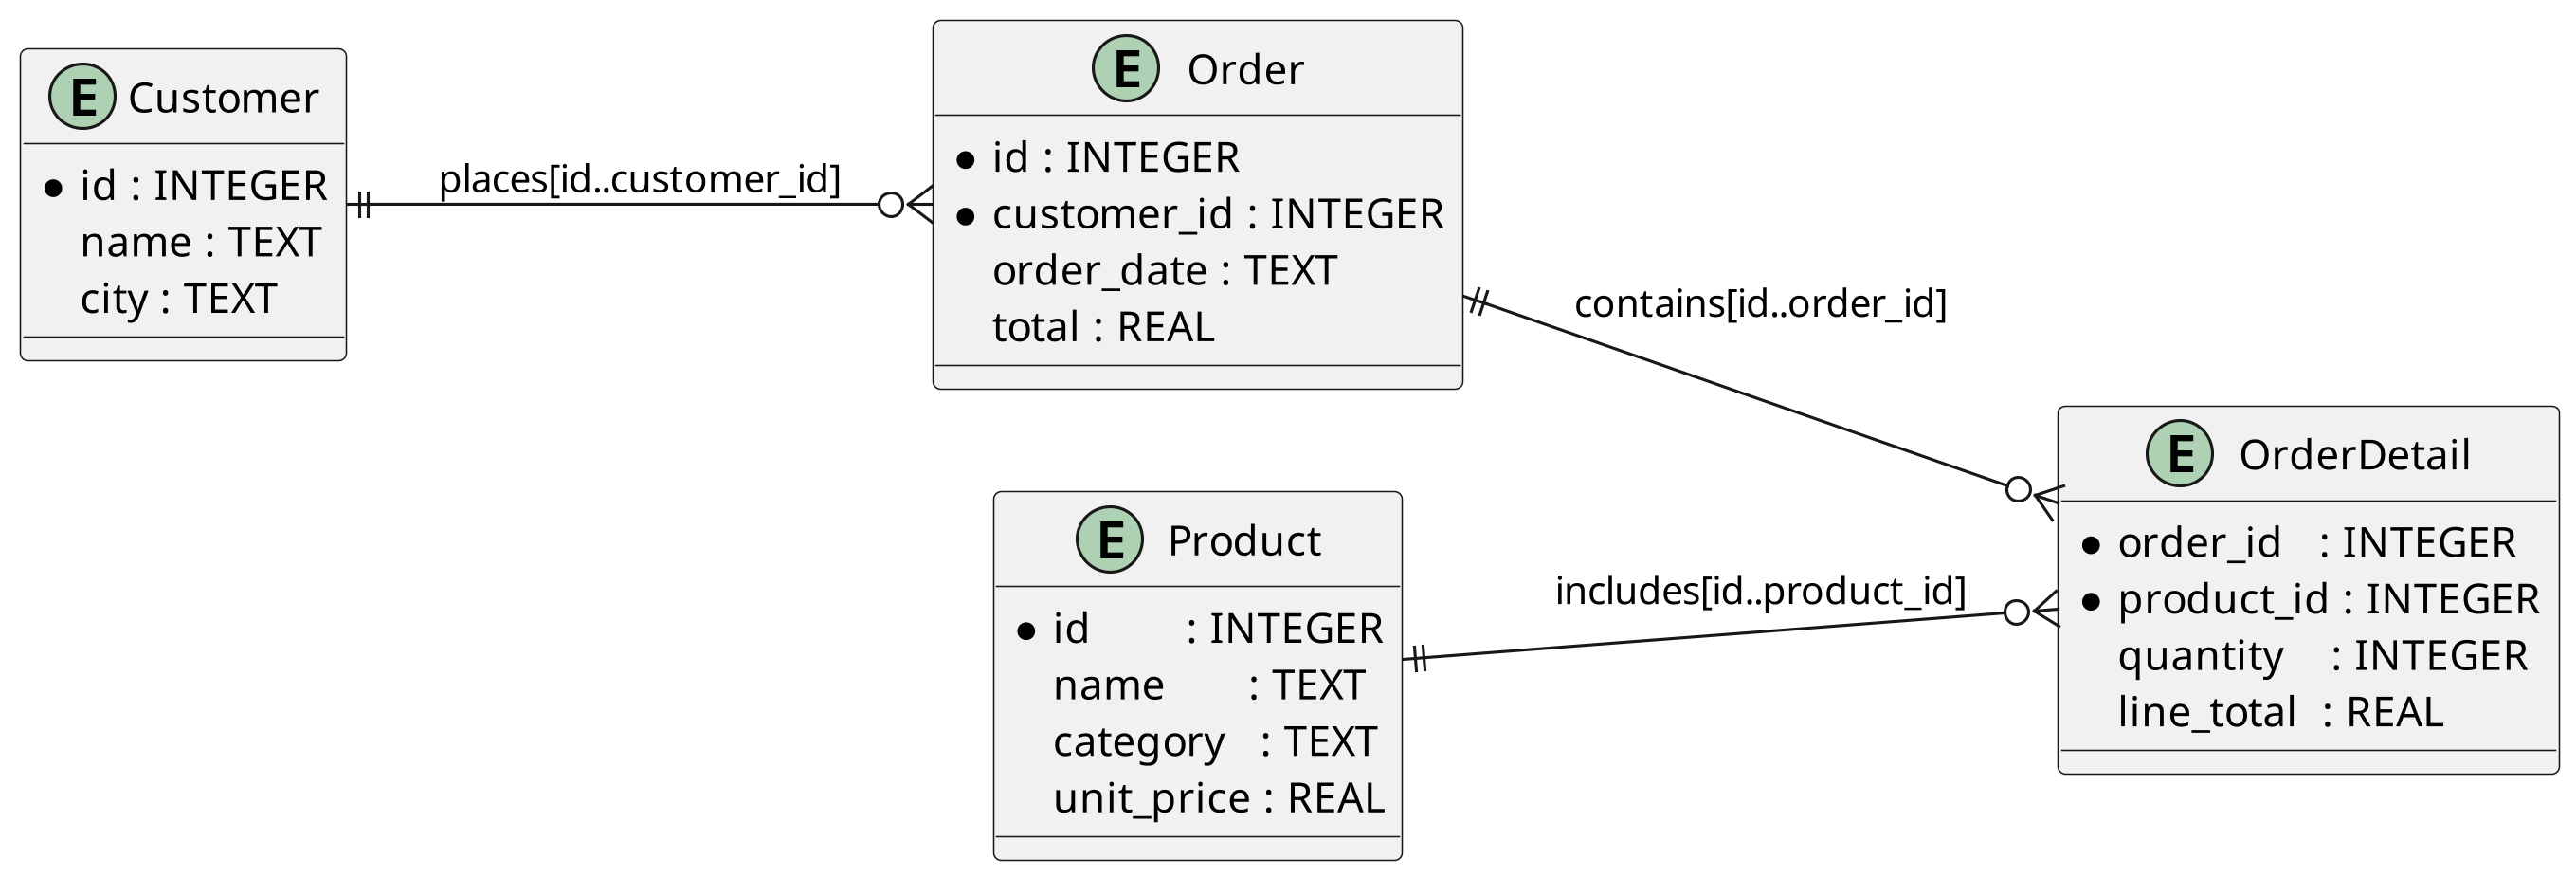
\includegraphics[width=\textwidth]{../slides/session04/data/out/erd.png}
	\caption{Diagram entitas–relasi Customer–Order–OrderDetail–Product dengan tipe data SQLite}
	\label{fig:customer_order_erd}
\end{figure}

\begin{itemize}
	\item Tabel \texttt{Order} memiliki atribut \texttt{customer\_id} yang menjadi \textbf{foreign key} mengarah ke \texttt{Customer.id}.
	\item Tabel \texttt{OrderDetail} memiliki dua foreign key: \texttt{order\_id} yang mengarah ke \texttt{Order.id}, dan \texttt{product\_id} yang mengarah ke \texttt{Product.id}.
\end{itemize}

Relasi ini memungkinkan kita untuk melakukan agregasi data lintas tabel, seperti menghitung total penjualan per pelanggan, mencari produk paling sering dipesan, atau menganalisis kota dengan performa pembelian tertinggi, menggunakan operasi \texttt{JOIN} dalam SQL.



\section{Demo Skema Relasional Sederhana}
\subsection{Alat Praktik: DB Browser}

Untuk mempermudah pemahaman dan praktik basis data relasional tanpa perlu instalasi server yang kompleks, kita menggunakan \textbf{DB Browser for SQLite}. Aplikasi ini menyediakan antarmuka grafis yang ringan untuk membuat, mengedit, dan menjalankan query SQL pada database SQLite.

DB Browser sangat cocok untuk sesi pembelajaran karena:
\begin{itemize}
	\item Gratis dan bersifat open source.
	\item Ringan dan tidak memerlukan setup database server.
	\item Menyediakan fitur drag-and-drop, visualisasi skema tabel, dan editor SQL.
\end{itemize}

\subsubsection{Langkah Instalasi DB Browser}

Langkah-langkah berikut dapat dilakukan pada sistem operasi Windows, macOS, maupun Linux:

\begin{enumerate}
	\item Buka situs resmi: \url{https://sqlitebrowser.org}.
	\item Klik menu \textbf{Download}, lalu pilih sesuai sistem operasi:
	\begin{itemize}
		\item Untuk Windows: \texttt{Standard installer for 64-bit Windows}.
		\item Untuk macOS: \texttt{DB Browser for SQLite.dmg}.
		\item Untuk Linux Ubuntu: jalankan perintah terminal \texttt{sudo apt install sqlitebrowser}.
	\end{itemize}
	\item Lakukan proses instalasi sesuai petunjuk masing-masing sistem.
\end{enumerate}

\subsubsection{Cara Menjalankan dan Menggunakan DB Browser}

Setelah proses instalasi selesai, lakukan langkah berikut untuk mulai membuat dan mengelola skema relasional:

\begin{enumerate}
\item Buka aplikasi \textbf{DB Browser for SQLite}.
\item Pilih menu \texttt{New Database} untuk membuat basis data baru.
\item Simpan file database dengan nama misalnya \texttt{ecommerce.db}.
\item Pilih tab \texttt{Execute SQL} untuk mulai mengetik perintah SQL.
\item Masukkan perintah SQL berikut untuk membuat tabel:

\begin{lstlisting}[style=SqlStyle]
CREATE TABLE customers (
	id INTEGER PRIMARY KEY AUTOINCREMENT,
	name TEXT,
	city TEXT
);

CREATE TABLE products (
	id INTEGER PRIMARY KEY AUTOINCREMENT,
	name TEXT,
	category TEXT,
	unit_price REAL
);

CREATE TABLE "orders" (
	id INTEGER PRIMARY KEY AUTOINCREMENT,
	customer_id INTEGER,
	order_date TEXT,
	total REAL,
	FOREIGN KEY (customer_id) REFERENCES customers(id)
);

CREATE TABLE order_details (
	id INTEGER PRIMARY KEY AUTOINCREMENT,
	order_id INTEGER,
	product_id INTEGER,
	quantity INTEGER,
	line_total REAL,
	FOREIGN KEY (order_id) REFERENCES "orders"(id),
	FOREIGN KEY (product_id) REFERENCES products(id)
);
\end{lstlisting}

\item Klik tombol \texttt{Play} atau \texttt{Execute All} untuk menjalankan perintah tersebut.
\item Buka tab \texttt{Browse Data} untuk melihat isi masing-masing tabel (yang masih kosong).
\item Gunakan kembali tab \texttt{Execute SQL} untuk mengisi data awal, contoh:

\begin{lstlisting}[language=SQL]
INSERT INTO customer (name, city) VALUES ('Andi', 'Jakarta');
INSERT INTO product (name, category, unit_price) 
	VALUES ('Mouse', 'Elektronik', 75000);
\end{lstlisting}

\end{enumerate}

\subsubsection{Fitur Tambahan untuk Praktik Lanjutan}

\begin{itemize}
\item Gunakan menu \texttt{Database Structure} untuk memverifikasi relasi antar tabel.
\item Untuk backup dan distribusi data, cukup salin file \texttt{.db} yang dibuat.
\item Untuk analisis, gunakan perintah SQL seperti \texttt{JOIN}, \texttt{GROUP BY}, dan \texttt{ORDER BY}.
\end{itemize}

Dengan DB Browser, pengguna dapat langsung fokus pada pemodelan data dan eksplorasi query SQL tanpa harus mengkonfigurasi layanan basis data yang kompleks.



\subsection{Menjawab Pertanyaan Penjualan}

Beberapa pertanyaan bisnis yang sering muncul dalam konteks e-commerce atau penjualan ritel antara lain:

\begin{itemize}
	\item Kota mana yang menghasilkan penjualan tertinggi?
	\item Pelanggan mana yang belum pernah melakukan pemesanan?
\item Kategori produk apa yang menyumbang pendapatan terbesar?
\end{itemize}

Contoh query untuk pelanggan yang belum pernah melakukan pemesanan:

\begin{lstlisting}[style=SqlStyle]
SELECT c.name FROM customers c
LEFT JOIN orders o ON c.id = o.customer_id
WHERE o.id IS NULL;
\end{lstlisting}

Penjelasan:
\begin{itemize}
\item \texttt{LEFT JOIN} memastikan semua pelanggan ditampilkan, termasuk yang tidak memiliki transaksi.
\item \texttt{WHERE o.id IS NULL} menyaring hanya pelanggan tanpa order.
\end{itemize}

Contoh query untuk mengetahui kota dengan penjualan tertinggi:

\begin{lstlisting}[style=SqlStyle]
SELECT c.city, SUM(o.total) AS total_sales
FROM customers c
JOIN orders o ON c.id = o.customer_id
GROUP BY c.city
ORDER BY total_sales DESC
LIMIT 5;
\end{lstlisting}

\textbf{Pertanyaan terjawab:} “Kota mana saja yang menghasilkan penjualan tertinggi?”

\subsection{Penggunaan GROUP BY, COUNT, dan LEFT JOIN}

Untuk menjawab pertanyaan berbasis agregasi digunakan kombinasi \texttt{GROUP BY} dan fungsi agregat seperti \texttt{SUM}, \texttt{COUNT}, atau \texttt{AVG}. Contoh lain:

\begin{lstlisting}[style=SqlStyle]
SELECT p.category, SUM(od.line_total) AS total_revenue
FROM order_details od
JOIN products p ON p.id = od.product_id
GROUP BY p.category
ORDER BY total_revenue DESC;
\end{lstlisting}

\textbf{Pertanyaan terjawab:} “Kategori produk apa yang menyumbang pendapatan terbesar?”

\subsection{Latihan Menjawab Pertanyaan Bisnis}

Tantangan mandiri untuk merancang dan menjalankan query:

\begin{enumerate}
\item Produk apa yang paling sering dibeli?
\item Pelanggan mana yang menyumbang total penjualan tertinggi?
\item Berapa rata-rata nilai transaksi per kota?
\item Apakah ada produk yang tidak pernah terjual?
\end{enumerate}

Contoh query untuk produk yang paling sering dibeli:

\begin{lstlisting}[style=SqlStyle]
SELECT p.name, SUM(od.quantity) AS total_quantity
FROM order_details od
JOIN products p ON p.id = od.product_id
GROUP BY p.name
ORDER BY total_quantity DESC
LIMIT 1;
\end{lstlisting}

Latihan bertujuan membekali kemampuan teknis mengekstraksi wawasan dari data dan mengembangkan pola pikir analitis berbasis data guna mendukung pengambilan keputusan manajerial.

\section{Jenis dan Perbandingan Produk RDBMS}

\subsection{Pengantar Sistem Manajemen Basis Data Relasional}

Sistem Manajemen Basis Data Relasional (Relational Database Management System, RDBMS) merupakan perangkat lunak yang dirancang untuk membuat, mengelola, dan mengakses data yang disimpan dalam bentuk relasional (tabel). Setiap tabel dalam sistem ini terdiri dari baris (record) dan kolom (field), serta memiliki relasi dengan tabel lain menggunakan konsep kunci primer dan kunci asing.

RDBMS memungkinkan integritas data, konsistensi, dan efisiensi pengambilan informasi dalam berbagai sistem informasi, mulai dari aplikasi keuangan, e-commerce, sistem logistik, hingga data warehouse dan big data analytics. RDBMS mendukung bahasa standar SQL (Structured Query Language) untuk manipulasi dan pemrosesan data.

\subsection{Perbandingan Produk RDBMS Populer}

Berbagai produk RDBMS tersedia di pasar dengan karakteristik berbeda-beda. Tabel \ref{tab:rdbms_comparison} merangkum beberapa RDBMS populer dan karakteristik utamanya:

\begin{table}[h]
	\centering
	\renewcommand{\arraystretch}{1.4}
	\begin{tabular}{|p{0.12\textwidth}|p{0.13\textwidth}|p{0.17\textwidth}|p{0.13\textwidth}|p{0.3\textwidth}|}
		\hline
		\textbf{Produk} & \textbf{Vendor} & \textbf{Tipe Lisensi} & \textbf{Skalabilitas} & \textbf{Penggunaan Umum} \\
		\hline
		MySQL & Oracle & Open Source / Komersial & Menengah–Tinggi & Aplikasi Web, CMS \\
		\hline
		PostgreSQL & Komunitas & Open Source & Tinggi & Data Analitik, Sistem ERP \\
		\hline
		SQLite & Komunitas & Open Source & Rendah–Menengah & Aplikasi Mobile, Embedded \\
		\hline
		SQL Server & Microsoft & Komersial & Tinggi & Sistem Enterprise, Keuangan \\
		\hline
		Oracle DB & Oracle & Komersial & Sangat Tinggi & Perbankan, ERP Skala Besar \\
		\hline
		MariaDB & MariaDB Foundation & Open Source & Menengah–Tinggi & Pengganti MySQL, Web Hosting \\
		\hline
	\end{tabular}
	\caption{Perbandingan Produk RDBMS Populer}
	\label{tab:rdbms_comparison}
\end{table}



Kriteria perbandingan meliputi lisensi, tingkat skalabilitas, serta bidang penerapan utama. SQLite, misalnya, cocok untuk aplikasi ringan dan perangkat bergerak, sedangkan Oracle Database dirancang untuk transaksi berskala besar dengan tingkat ketersediaan dan keamanan tinggi.

\subsection{Aspek: Lisensi dan Biaya (Open Source vs Komersial)}

Produk RDBMS dapat dibedakan berdasarkan jenis lisensi dan model biaya:

\begin{itemize}
	\item \textbf{Open Source:} seperti PostgreSQL, SQLite, dan MariaDB, tersedia bebas untuk digunakan dan dimodifikasi. Cocok untuk pengembangan aplikasi, lingkungan akademik, serta organisasi dengan anggaran terbatas.
	\item \textbf{Komersial:} seperti Oracle Database dan Microsoft SQL Server, menawarkan fitur tambahan seperti keamanan canggih, replikasi terdistribusi, high availability, dan dukungan teknis resmi. Lisensi bersifat berbayar dengan skema per CPU core, per user, atau per subscription.
	\item \textbf{Hybrid:} beberapa produk seperti MySQL menyediakan edisi komunitas (gratis) dan edisi enterprise (berbayar) dengan fitur tambahan dan SLA.
\end{itemize}

Pemilihan RDBMS sebaiknya mempertimbangkan faktor biaya total kepemilikan (Total Cost of Ownership), kebutuhan performa, volume transaksi, serta dukungan komunitas atau vendor.

\subsection{Aspek: Kinerja dan Skalabilitas}

Kinerja dan skalabilitas merupakan aspek penting dalam memilih sistem manajemen basis data relasional (RDBMS), khususnya pada skenario bisnis dengan volume transaksi tinggi dan permintaan waktu respons cepat. Kinerja mengacu pada seberapa cepat sistem dapat mengeksekusi query, sedangkan skalabilitas merujuk pada kemampuan sistem menangani peningkatan beban kerja secara efisien.

Beberapa RDBMS seperti \textbf{PostgreSQL} dan \textbf{Oracle Database} menawarkan optimisasi query lanjutan dan kemampuan parallel processing. \textbf{MySQL} dikenal cukup efisien untuk aplikasi berskala kecil hingga menengah, namun memiliki keterbatasan dalam penanganan workload analitik kompleks secara default. \textbf{SQL Server} memiliki engine yang dioptimalkan untuk integrasi dengan sistem Microsoft lainnya, dan dapat diskalakan secara vertikal maupun horizontal melalui fitur seperti Always On dan Database Sharding.

Sementara itu, \textbf{SQLite} dirancang untuk kinerja tinggi dalam skenario lokal atau embedded, tetapi tidak cocok untuk penggunaan dengan volume data besar dan akses bersamaan (concurrency) tinggi.

Faktor yang perlu dipertimbangkan:
\begin{itemize}
	\item Kemampuan indexing, partitioning, dan caching
	\item Mekanisme concurrency control (MVCC, locking)
	\item Performa join dan subquery pada skala besar
\end{itemize}

\subsection{Aspek: Dukungan Cloud dan Vendor Lock-in}

Dukungan terhadap infrastruktur cloud telah menjadi kriteria utama dalam pemilihan RDBMS modern. Banyak organisasi memilih solusi database yang siap digunakan di layanan cloud publik seperti Amazon Web Services (AWS), Google Cloud Platform (GCP), dan Microsoft Azure.

Beberapa opsi populer:

\begin{itemize}
	\item \textbf{Amazon RDS}: mendukung MySQL, PostgreSQL, MariaDB, SQL Server, dan Oracle.
	\item \textbf{Google Cloud SQL}: fokus pada PostgreSQL dan MySQL.
	\item \textbf{Azure SQL Database}: versi fully-managed dari Microsoft SQL Server di cloud.
\end{itemize}

Meskipun solusi cloud memudahkan pengelolaan dan penskalaan, penggunaan produk-produk tertentu dapat menimbulkan risiko \textit{vendor lock-in} — yaitu ketergantungan terhadap satu penyedia layanan. Hal ini dapat menyulitkan migrasi di masa depan karena perbedaan fitur, lisensi, atau format penyimpanan data.

Mitigasi vendor lock-in dapat dilakukan dengan:
\begin{itemize}
	\item Memilih RDBMS open source yang didukung oleh banyak platform
	\item Menggunakan standar SQL tanpa ekstensi khusus vendor
	\item Mendesain arsitektur dengan layer abstraction untuk fleksibilitas
\end{itemize}

\subsection{Pemilihan RDBMS Berdasarkan Kebutuhan Bisnis}

Pemilihan produk RDBMS sebaiknya mempertimbangkan profil kebutuhan spesifik dari organisasi atau unit bisnis. Tidak ada satu sistem yang cocok untuk semua skenario, sehingga keputusan perlu didasarkan pada sejumlah parameter berikut:

\begin{itemize}
	\item \textbf{Volume dan jenis data:} untuk data terstruktur yang besar dan kompleks, PostgreSQL dan Oracle lebih unggul. Untuk aplikasi ringan, SQLite atau MySQL cukup memadai.
	\item \textbf{Jenis transaksi:} sistem dengan banyak transaksi simultan memerlukan dukungan concurrency tinggi seperti pada SQL Server dan PostgreSQL.
	\item \textbf{Integrasi sistem:} untuk organisasi dengan ekosistem Microsoft, SQL Server menjadi pilihan alami.
	\item \textbf{Anggaran dan lisensi:} PostgreSQL dan MariaDB menawarkan solusi tanpa biaya lisensi, cocok untuk organisasi dengan keterbatasan anggaran.
	\item \textbf{Kebutuhan analitik:} PostgreSQL dengan ekstensi seperti TimescaleDB atau Apache AGE mendukung time-series dan graph analytics.
\end{itemize}

Evaluasi kebutuhan dan konteks bisnis memungkinkan pengambilan keputusan teknologi yang lebih rasional, efektif, dan berkelanjutan dalam jangka panjang.

\section{Data Terstruktur/Basis Data Relasional dengan Big Data}

\subsection{Posisi Data Terstruktur dalam Arsitektur Big Data}

Dalam arsitektur big data modern, data terstruktur tetap memiliki peran penting meskipun data semi-terstruktur dan tidak terstruktur makin mendominasi. Data terstruktur mengacu pada data yang tersimpan dalam format tabular seperti baris dan kolom, dengan skema yang konsisten, seperti yang terdapat pada sistem basis data relasional (RDBMS). Contoh sumber data terstruktur antara lain: sistem transaksi penjualan, data keuangan, sistem kepegawaian, atau catatan layanan pelanggan.

Dalam kerangka arsitektur big data, data terstruktur biasanya ditempatkan pada \textit{structured zone} atau \textit{trusted layer}, setelah melalui proses ingest dari berbagai sumber. Pada sistem data lake modern, seperti yang didukung oleh AWS Lake Formation atau Azure Data Lake, zona terstruktur digunakan untuk penyimpanan data yang telah dibersihkan, dikurasi, dan siap untuk query analitik \cite{giebler2020structured}.

RDBMS tradisional seringkali kurang efisien untuk volume data sangat besar, sehingga banyak organisasi memanfaatkan teknologi seperti Apache Hive, Apache Impala, atau Presto yang mendukung eksekusi query SQL pada skala petabyte di atas Hadoop Distributed File System (HDFS) atau Amazon S3. Sistem ini menggabungkan fleksibilitas penyimpanan big data dengan kekuatan ekspresif bahasa SQL untuk data terstruktur \cite{armbrust2015spark}.

\subsection{Peran SQL dalam Proses ETL dan Big Data}

SQL tetap menjadi alat utama dalam proses ETL (Extract, Transform, Load), baik dalam sistem tradisional maupun ekosistem big data. Pada fase \textbf{Extract}, SQL digunakan untuk mengambil data dari berbagai sumber RDBMS atau file CSV. Pada fase \textbf{Transform}, SQL membantu dalam pembersihan, pemrosesan, agregasi, penggabungan antar tabel, dan pembuatan tabel dimensi atau fakta yang siap dianalisis. Pada fase \textbf{Load}, hasil transformasi diunggah kembali ke warehouse atau data lake.

Platform big data modern seperti Apache Spark, Google BigQuery, dan Snowflake menyediakan SQL engine yang memungkinkan proses transformasi kompleks dilakukan langsung di atas data berukuran besar tanpa harus mengekstraknya secara manual. Spark SQL, misalnya, memungkinkan pemrosesan data paralel berbasis SQL di atas kumpulan data besar, sekaligus menyediakan interoperabilitas dengan Python atau Scala \cite{zaharia2016spark}. Hal ini menjadikan SQL sebagai jembatan antara dunia relasional dan paradigma big data.

Dengan adopsi standar seperti ANSI SQL dan integrasi SQL ke dalam sistem big data, penguasaan SQL tetap menjadi keterampilan kunci untuk profesional analitik dan manajerial di era data skala besar.


\section{Kesimpulan}

Pemahaman terhadap data terstruktur dan basis data relasional merupakan fondasi penting dalam pengelolaan data modern, termasuk dalam konteks big data. Dengan mengenal konsep dasar seperti tabel, kolom, baris, kunci primer dan kunci asing, serta relasi antarentitas seperti pelanggan, pesanan, dan produk, pelaku bisnis dan manajer dapat lebih mudah memahami struktur penyimpanan data yang menjadi sumber informasi penting dalam pengambilan keputusan. SQL sebagai bahasa query utama menyediakan cara sistematis dan efisien untuk mengekstrak, menganalisis, dan mengelola data terstruktur tersebut.

Dalam konteks arsitektur big data, data terstruktur tetap memainkan peran sentral terutama dalam zona-zona terkurasi dan proses ETL. Berbagai sistem seperti Apache Hive, Spark SQL, dan layanan cloud modern memungkinkan eksekusi query SQL pada skala besar. Oleh karena itu, keterampilan dalam memahami struktur data relasional dan mengoperasikan SQL tidak hanya relevan untuk teknisi, tetapi juga menjadi kompetensi penting bagi profesional bisnis yang ingin memanfaatkan data sebagai aset strategis.


